\chapter{Erklärung zum Einsatz von KI-gestützten Werkzeugen}

Im Rahmen der Erstellung dieser Bachelorarbeit wurden KI-gestützte Werkzeuge
eingesetzt. Die nachfolgende Tabelle gibt einen Überblick über die verwendeten
Systeme sowie deren jeweiligen Einsatzbereich.

\begin{table}[htbp]
    \centering
  \begin{tabular}{p{3.5cm} p{3.5cm} p{5cm}}
    \toprule
    \textbf{Werkzeug} & \textbf{Anbieter} & \textbf{Verwendungszweck} \\
    \midrule
    Claude Sonnet 4.6 & Anthropic & Unterstützung bei der sprachlichen
                                   Formulierung von Textpassagen und Unterstützung des Quellcodes \\
    \addlinespace
    Perplexity       & Perplexity AI & Recherche und Identifikation
                                       wissenschaftlicher Quellen \\
    \addlinespace
    DeepL             & DeepL SE & Übersetzung von Textpassagen und
                                   Fachbegriffen \\
    \bottomrule
  \end{tabular}
  \caption{Eingesetzte KI-gestützte Werkzeuge}
  \label{tab:ki-werkzeuge}
\end{table}

Sämtliche durch KI-Werkzeuge generierten oder unterstützten Inhalte wurden
kritisch geprüft, überarbeitet und eigenverantwortlich in die Arbeit integriert.
Die inhaltliche Verantwortung für alle Aussagen dieser Arbeit liegt
ausschließlich bei der Verfasserin bzw. dem Verfasser.

\chapter{Zusätzliche Abbildungen}
\label{appendix:abbildungen}
\clearpage
\begin{figure}[H]
     \centering
     \includesvg[width=1.0\linewidth]{figures/authentication-screens.svg}
     \caption{Implementierte Screens für die Authentifizierung}
     \label{fig:anhang_authentication}
 \end{figure}

 \begin{figure}[H]
     \centering
     \includesvg[width=1.0\linewidth]{figures/tab-light-screens.svg}
     \caption{Implementierte Screens der Tabs in Light Theme}
     \label{fig:anhang_tab-light}
 \end{figure}

 \begin{figure}[H]
     \centering
     \includesvg[width=1.0\linewidth]{figures/tab-dark-screens.svg}
     \caption{Implementierte Screens der Tabs in Dark Theme}
     \label{fig:anhang_tab-dark}
 \end{figure}

 \begin{figure}[H]
     \centering
     \includesvg[width=1.0\linewidth]{figures/booking-process-screens.svg}
     \caption{Implementierte Screens des Buchungsprozesses}
     \label{fig:anhang_booking-process}
 \end{figure}

\chapter{Fragebogen der Nutzerstudie}
\label{appendix:fragebogen}

Der folgende Fragebogen wurde im Rahmen der aufgabenbasierten Nutzerstudie
eingesetzt. Die Teilnehmenden füllten ihn im Anschluss an die vier Aufgaben
über Google Forms aus. Der Fragebogen umfasst insgesamt 33 Fragen und gliedert
sich in fünf Abschnitte.

\section*{Abschnitt 1: Allgemeine App-Erfahrung}
\begin{figure}[H]
    \centering
    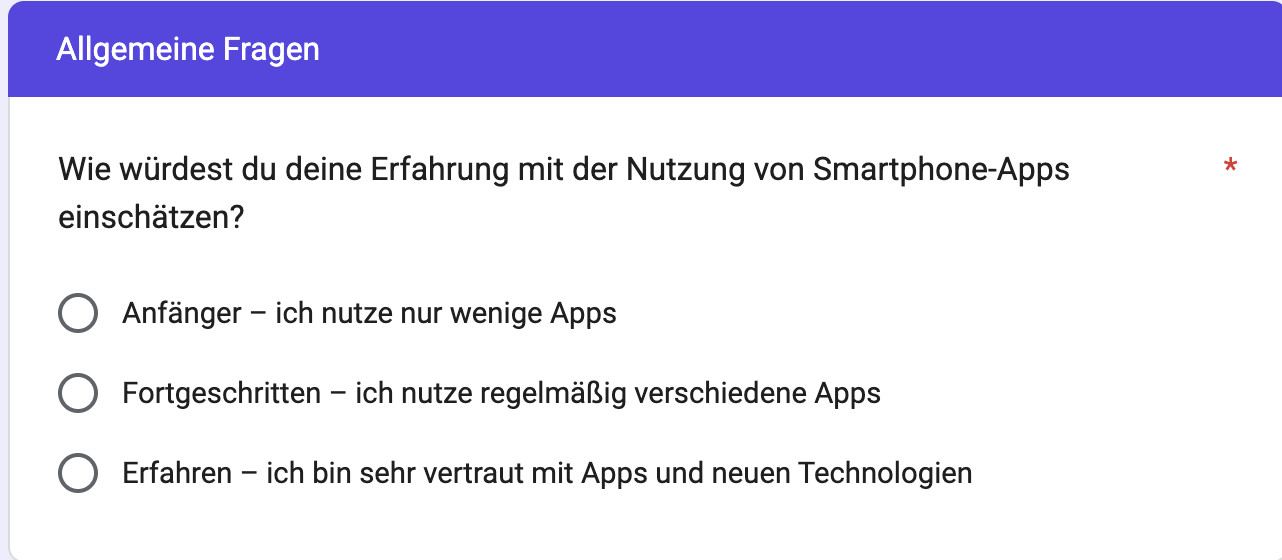
\includegraphics[width=1.0\linewidth]{figures/evaluation/allgemeine_fragen.png}
\end{figure}

\section*{Abschnitt 2: Aufgabenbezogene Fragen}

Die folgenden Fragen beziehen sich auf die vier Aufgaben der Studie.

\begin{figure}[H]
    \centering
    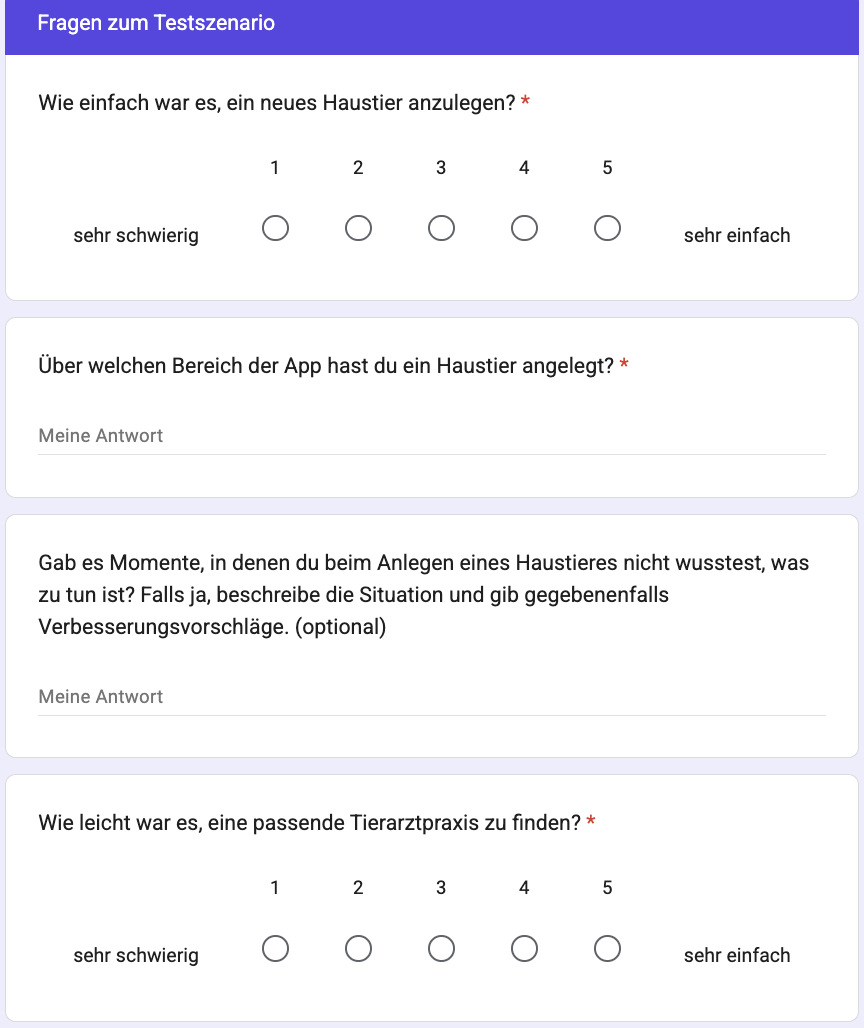
\includegraphics[width=1.0\linewidth]{figures/evaluation/Aufgaben_1.png}
\end{figure}

\begin{figure}[H]
    \centering
    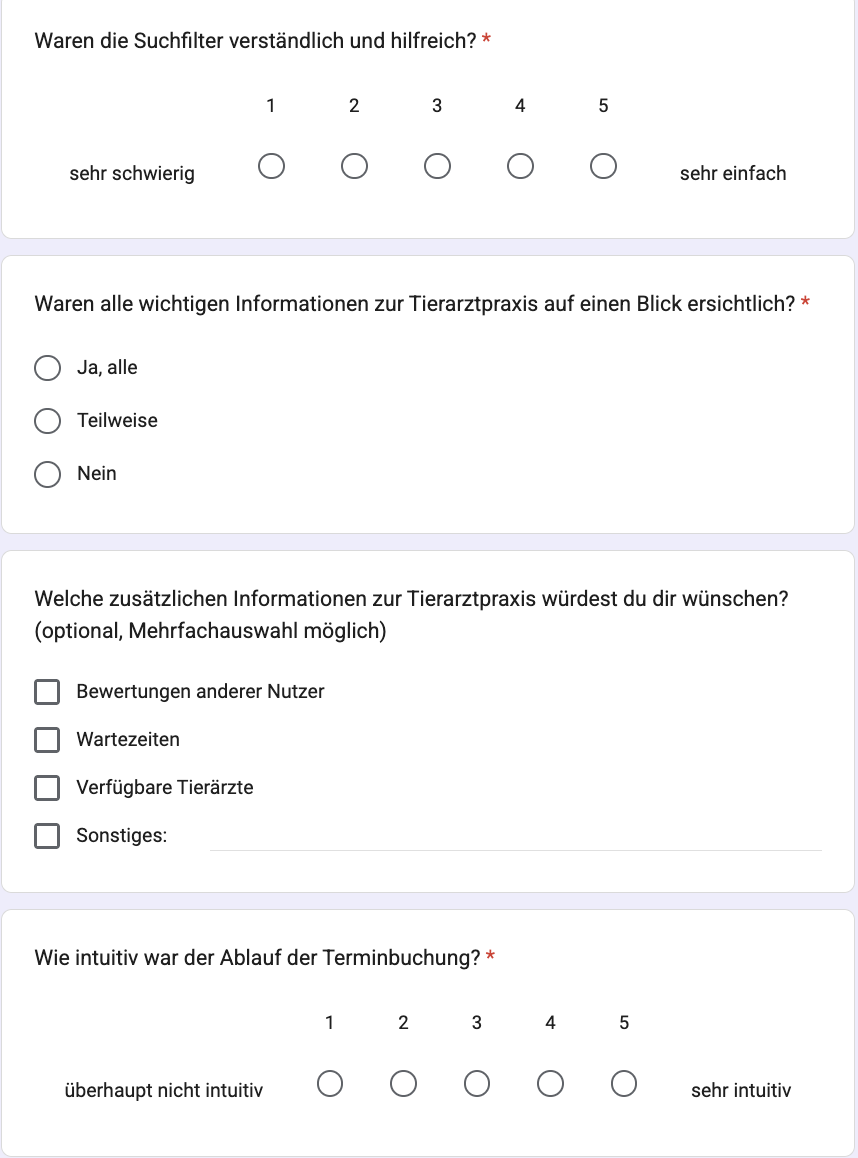
\includegraphics[width=1.0\linewidth]{figures/evaluation/Aufgaben_2.png}
\end{figure}

\begin{figure}[H]
    \centering
    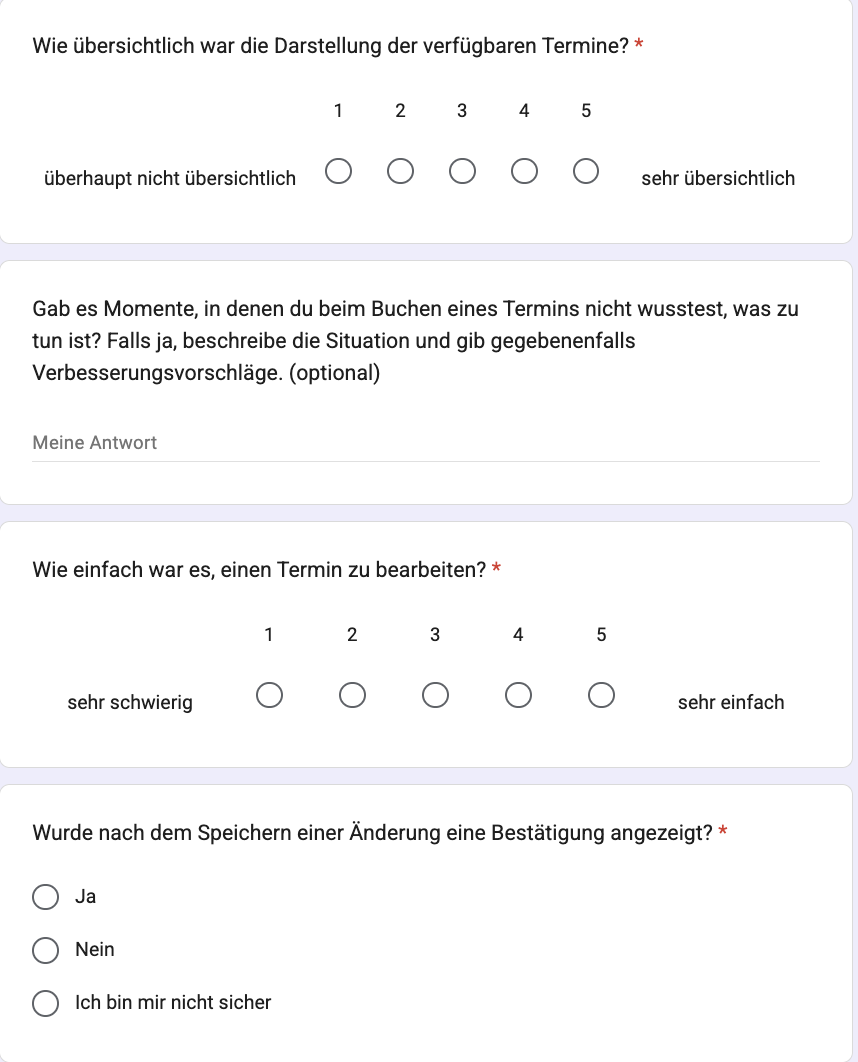
\includegraphics[width=1.0\linewidth]{figures/evaluation/Aufgaben_3.png}
\end{figure}

\begin{figure}[H]
    \centering
    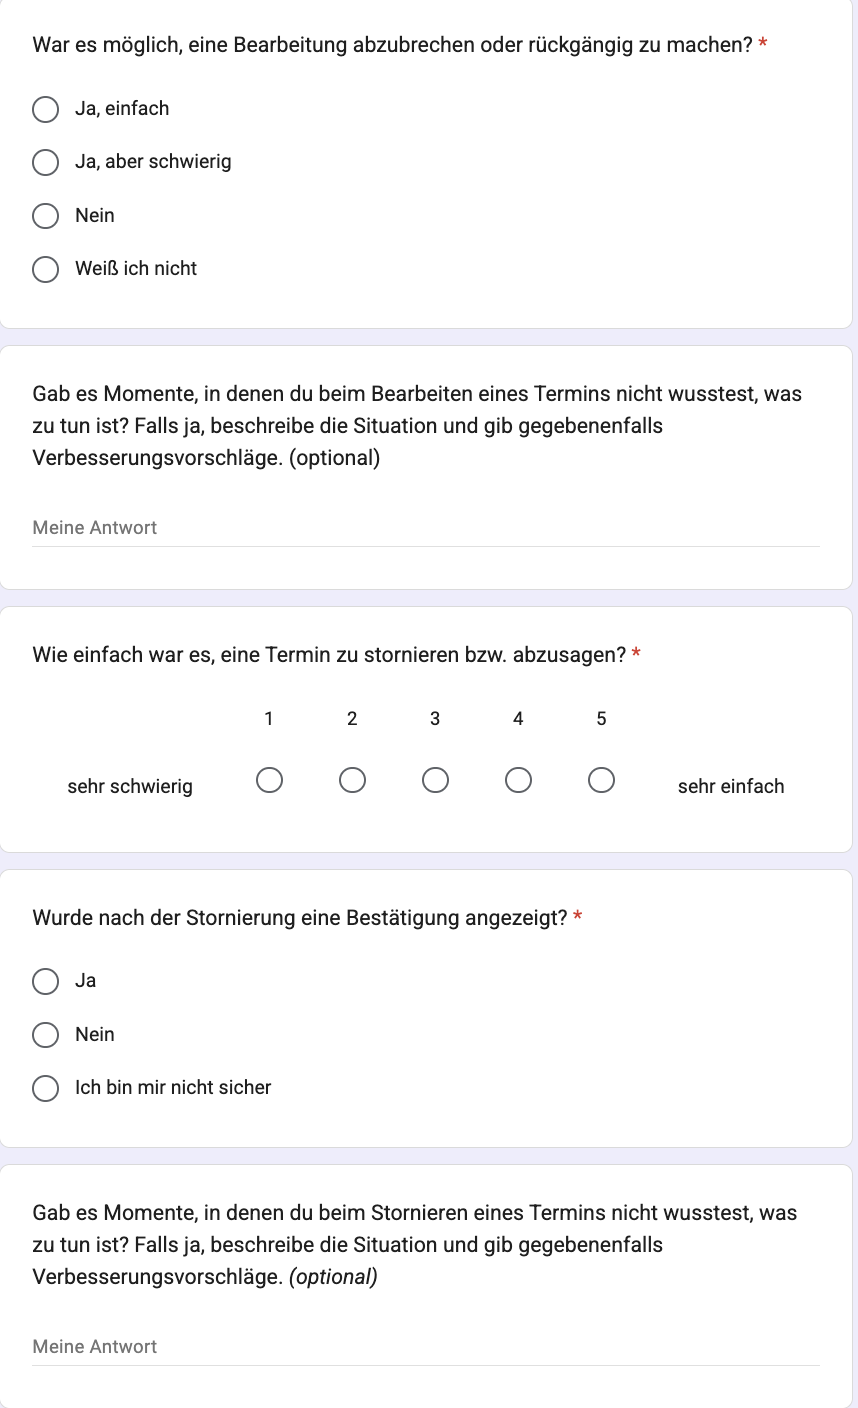
\includegraphics[width=1.0\linewidth]{figures/evaluation/Aufgaben_4.png}
\end{figure}

\section*{Abschnitt 3: System Usability Scale}

Die folgenden Fragen beziehen sich auf die Benutzerfreundlichkeit der Anwendung.

\begin{figure}[H]
    \centering
    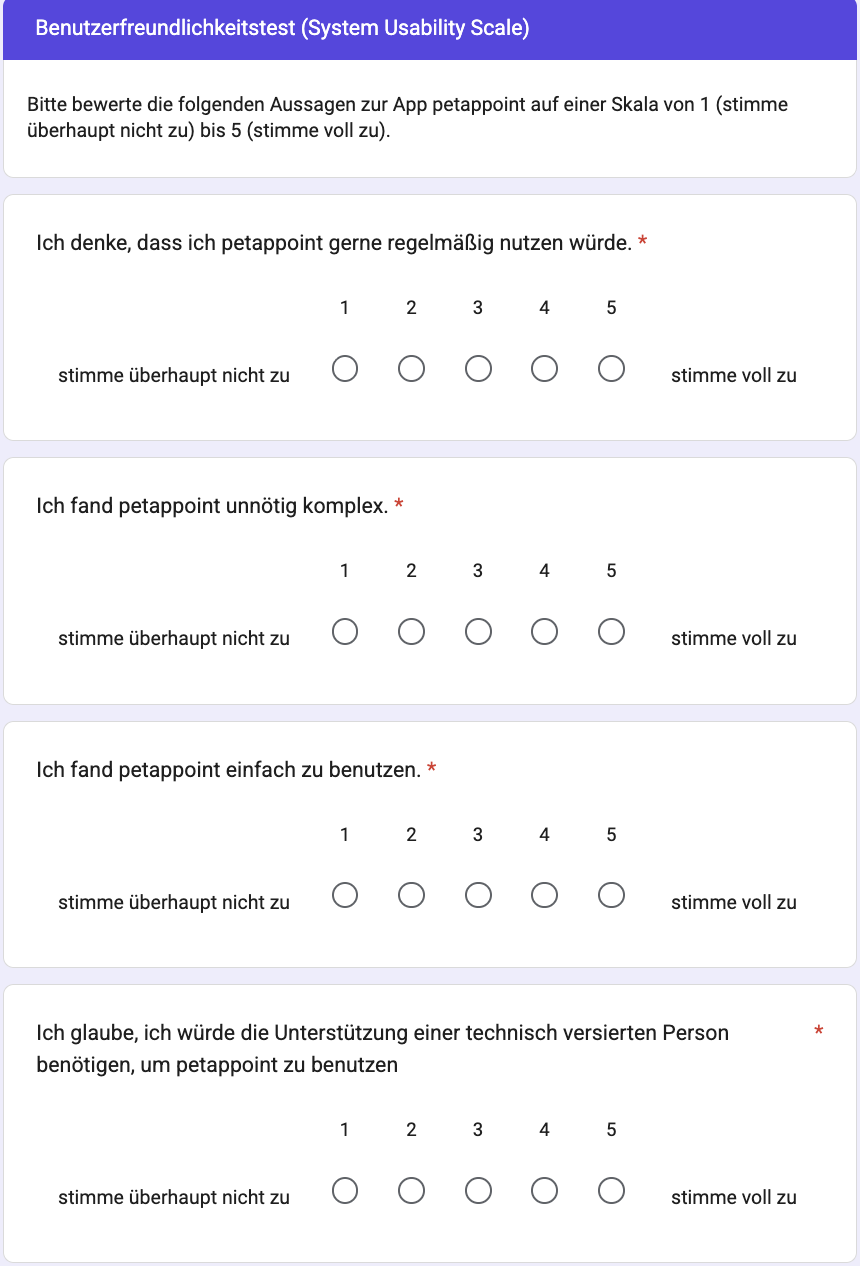
\includegraphics[width=1.0\linewidth]{figures/evaluation/Sus_1.png}
\end{figure}

\begin{figure}[H]
    \centering
    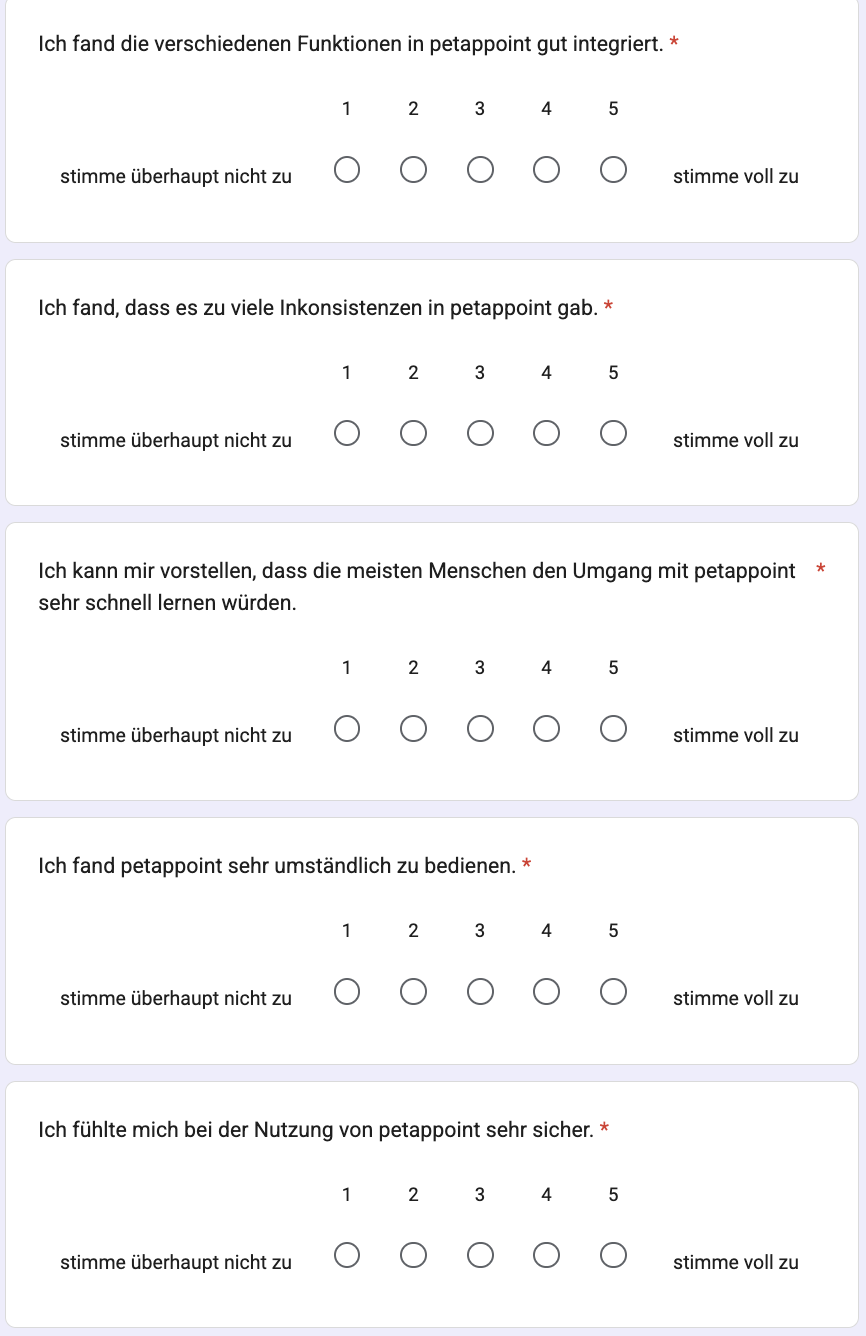
\includegraphics[width=1.0\linewidth]{figures/evaluation/Sus_2.png}
\end{figure}

\begin{figure}[H]
    \centering
    \includegraphics[width=1.0\linewidth]{figures/evaluation/Sus_3.png}
\end{figure}

\section*{Abschnitt 4: Plattformwahrnehmung}

Die folgenden Fragen beziehen sich auf die Plattformwahrnehmung der Anwendung.
\begin{figure}[H]
    \centering
    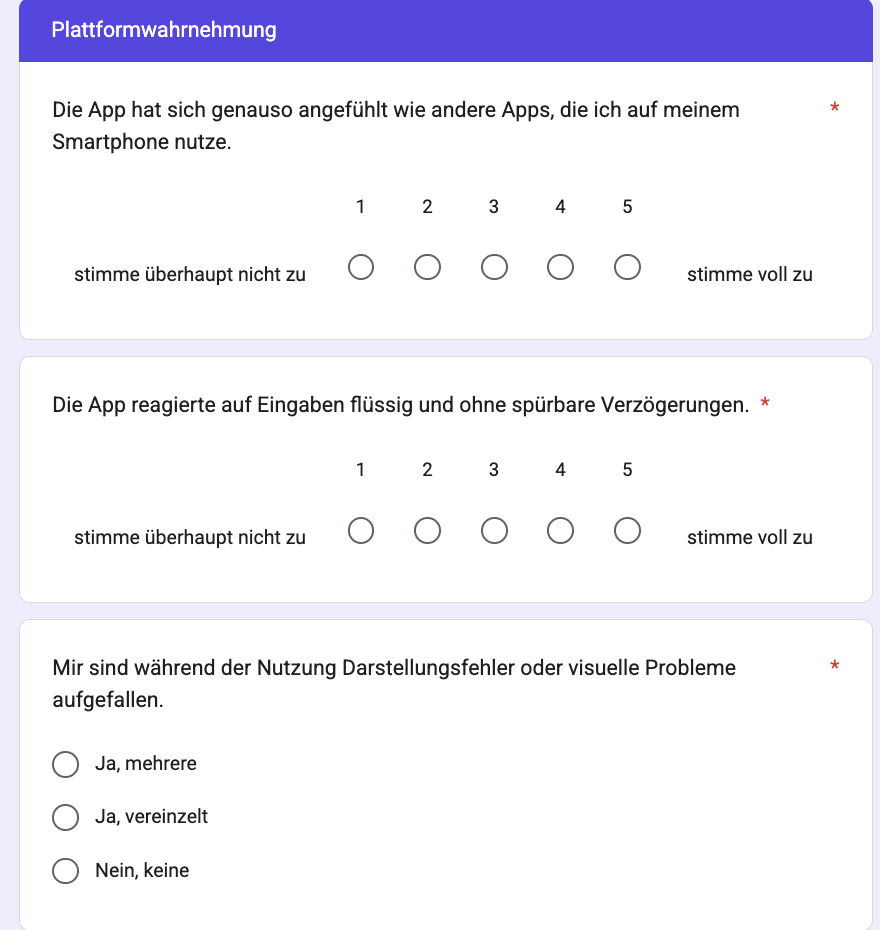
\includegraphics[width=1.0\linewidth]{figures/evaluation/Plattformwahrnehmung_1.png}
\end{figure}

\section*{Abschnitt 5: Offene Fragen}

Die folgenden offenen Fragen geben den Teilnehmenden die Möglichkeit, freies Feedback zur Anwendung zu geben.

\begin{figure}[H]
    \centering
    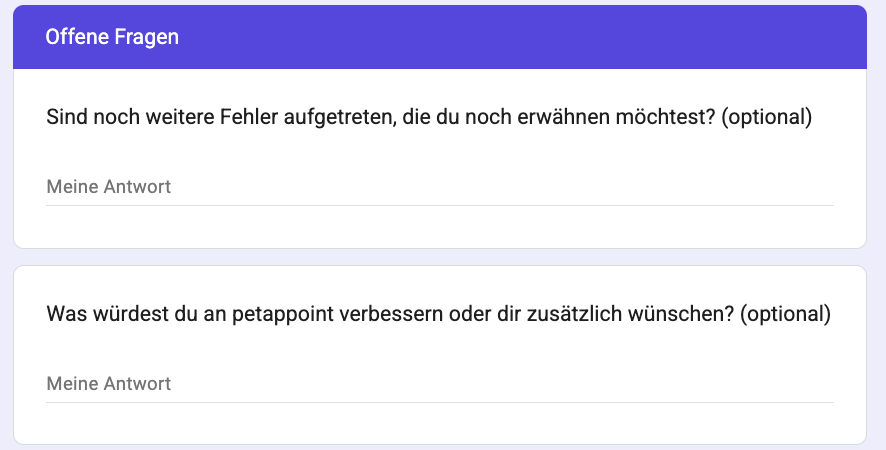
\includegraphics[width=1.0\linewidth]{figures/evaluation/offene_fragen.png}
\end{figure}


\chapter{Rohdaten der Nutzerstudie}
\label{appendix:rohdaten}
Die vollständigen Rohdaten der Nutzerstudie sind als CSV-Datei über folgenden Link abrufbar:
\begin{itemize}
  \item Fragebogenantworten (CSV): \\
\url{https://drive.google.com/file/d/1mYSi_oevs_g2PIkNzhTzI93mcST8AHD-/view?usp=sharing}
  \item Alter, Beruf und Aufgabenzeiten (Excel): \\
        \url{https://docs.google.com/spreadsheets/d/1hDo-o8bUvvBQezd9emxWkkEGwxBhKNbc/edit?usp=sharing&ouid=107616586787460661537&rtpof=true&sd=true}
  \item SUS-Scores jedes einzelnen Teilnehmer(Excel): \\
        \url{https://docs.google.com/spreadsheets/d/1hy-Kzu3R7k8lXaasbQmuu2rEZsG50OkU/edit?usp=sharing&ouid=107616586787460661537&rtpof=true&sd=true}
\end{itemize}